%!TEX root = ../../thesis.tex

\ac{ggF} is modelled by \meps{\powhegbox}{\pythia{8}}, including the exact mass 
dependence of the \Ptop and \Pbottom quarks in the loop \cite{Powheg-ggF-quarkmasses}. 
The \powhegbox parameter \verb|hfact| controls the scale at which the emission 
transitions from Sudakov-like to ME-like. This is tuned to $\mH/1.2$ in order to 
reproduce the Higgs boson \pt distribution of \hqt \cite{HqT2} (NLO+NNLL accuracy). This 
tuning is further discussed in \Section~4.9 of \Reference \cite{YR2}.



\subsection{Higgs boson transverse momentum}
\todo[inline]{Include Higgs \pt studies?}



\subsection{Event selection acceptance}

In \Section~\ref{sec:ggf_jetbin}, perturbative uncertainties in the jet binning were 
considered. The jet bin fractions predicted by MC were found to be in agreement with the 
dedicated jet-binned cross section calculations. 

We now consider uncertainties in the acceptance of the event selection. These are 
evaluated at hadron-level (\ie before detector simulation) by changing some aspect of 
the MC modelling and measuring the effect upon the acceptance. The selection criteria are 
very similar to those applied at detector-level, and are summarised in 
\Table~\ref{tab:signal:acc_truthselection}.

The hadron-level object definitions follow. The MC event record is used to identify 
leptons and neutrinos which descend from the Higgs boson. An \metvec vector is 
constructed from the neutrinos. Each lepton is `dressed' with the four-momenta of photons 
within a cone of $\Delta R < 0.1$, in order to recover energy lost via QED FSR. Jets are 
found using individual particles as inputs (\cf topo-clusters at detector-level). Muons 
and neutrinos are excluded from jet finding since they interact weakly with the 
calorimeter. Leptons and jets are required to pass the same \pt and $\eta$ criteria 
applied at detector-level.

\begin{table}
	\begin{tabular}{ccc}
		Jet binning & \ee/\mm & \em/\me \\
		\hline
		Inclusive & \multicolumn{2}{c}{Exactly 2 opposite-sign leptons} \\
		& \multicolumn{2}{c}{\unit{$\ptleadlep > 22$}{\GeV}} \\
		& \unit{$\mll > 12$}{\GeV} & \unit{$\mll > 10$}{\GeV} \\
		& \unit{$\mods{\mll - \mZ} > 15$}{\GeV} & -- \\
		\hline
		0-jet & \unit{$\metrel > 40$}{\GeV} & \unit{$\met > 20$}{\GeV} \\
		& \multicolumn{2}{c}{$\dphillmet > 1.57$} \\
		& \multicolumn{2}{c}{\unit{$\ptll > 30$}{\GeV}} \\
		& \multicolumn{2}{c}{\unit{$\mll < 55$}{\GeV}} \\
		& \multicolumn{2}{c}{$\dphill < 1.8$} \\
		\hline
		1-jet & \unit{$\metrel > 40$}{\GeV} & \unit{$\met > 10$}{\GeV} \\
		& -- & \unit{$\maxmtw > 50$}{\GeV} \\
		& -- & \unit{$\mtautau < 66$}{\GeV} \\
		& \multicolumn{2}{c}{\unit{$\mll < 55$}{\GeV}} \\
		& \multicolumn{2}{c}{$\dphill < 1.8$} \\
		\hline
		\twojet & \unit{$\met > 45$}{\GeV} & \unit{$\met > 20$}{\GeV} \\
		& \multicolumn{2}{c}{\unit{$\mtautau < 66$}{\GeV}} \\
		& \multicolumn{2}{c}{Fails $\dyjj > 3.6$ or \unit{$\mjj > 600$}{\GeV} or CJV or OLV} \\
		& \multicolumn{2}{c}{\unit{$\mll < 55$}{\GeV}} \\
		& \multicolumn{2}{c}{$\dphill < 1.8$} \\
	\end{tabular}
	\caption{Hadron-level event selection used to calculate ggF acceptance uncertainties. 
	The CJV and OLV are the central jet veto and outside lepton veto, respectively. See 
	\Chapter~\ref{chap:selection} for a detailed explanation of the criteria.}
	\label{tab:signal:acc_truthselection}
\end{table}

\begin{table}
	\begin{tabular}{cc|ccccccc}
		\multirow{2}{*}{Channel} & \multirow{2}{*}{Jet bin} & \multirow{2}{*}{Scale} & CT10 vs & CT10 & Py8 vs & Py8 vs & Powheg vs & \multirow{2}{*}{Total} \\
		&  &  & MSTW & error sets & Py6 & Jimmy & MC$@$NLO \\
		\hline
		\ee/\mm &   0-jet & 1.4\% & +1.9\% & 5.3\% & $+1.6\%$ & $+6.4\%$ & $+5.1\%$ \\
		\em/\me &   0-jet & 1.1\% & +1.9\% & 5.3\% & $-0.5\%$ & $+2.2\%$ & $+1.3\%$ \\
		\ee/\mm &   1-jet & 1.9\% & +1.8\% & 4.6\% & $-0.7\%$ & $+2.1\%$ & $+2.3\%$ \\
		\em/\me &   1-jet & 1.3\% & +1.8\% & 4.7\% & $+0.5\%$ & $+3.5\%$ & $+3.6\%$ \\
		\ee/\mm & \twojet &       & +2.0\% & 3.7\% & $+0.8\%$ & $-1.0\%$ & $-5.6\%$ \\
		\em/\me & \twojet &       & +2.0\% & 3.6\% & $-0.5\%$ & $+1.5\%$ & $-2.9\%$ \\
	\end{tabular}
	\caption{Theoretical uncertainties in the acceptance of ggF in each signal 
	region, split by opposite/same flavour channels and jet bins. PDF uncertainties are
	evaluated for acceptances relative to the inclusive cross section, whereas others are
	calculated within jet bins.}
	\label{tab:signal:acc_unc_small}
\end{table}


\subsection{\mt shape modelling}



\subsection{ME-PS matching}

\begin{figure}
	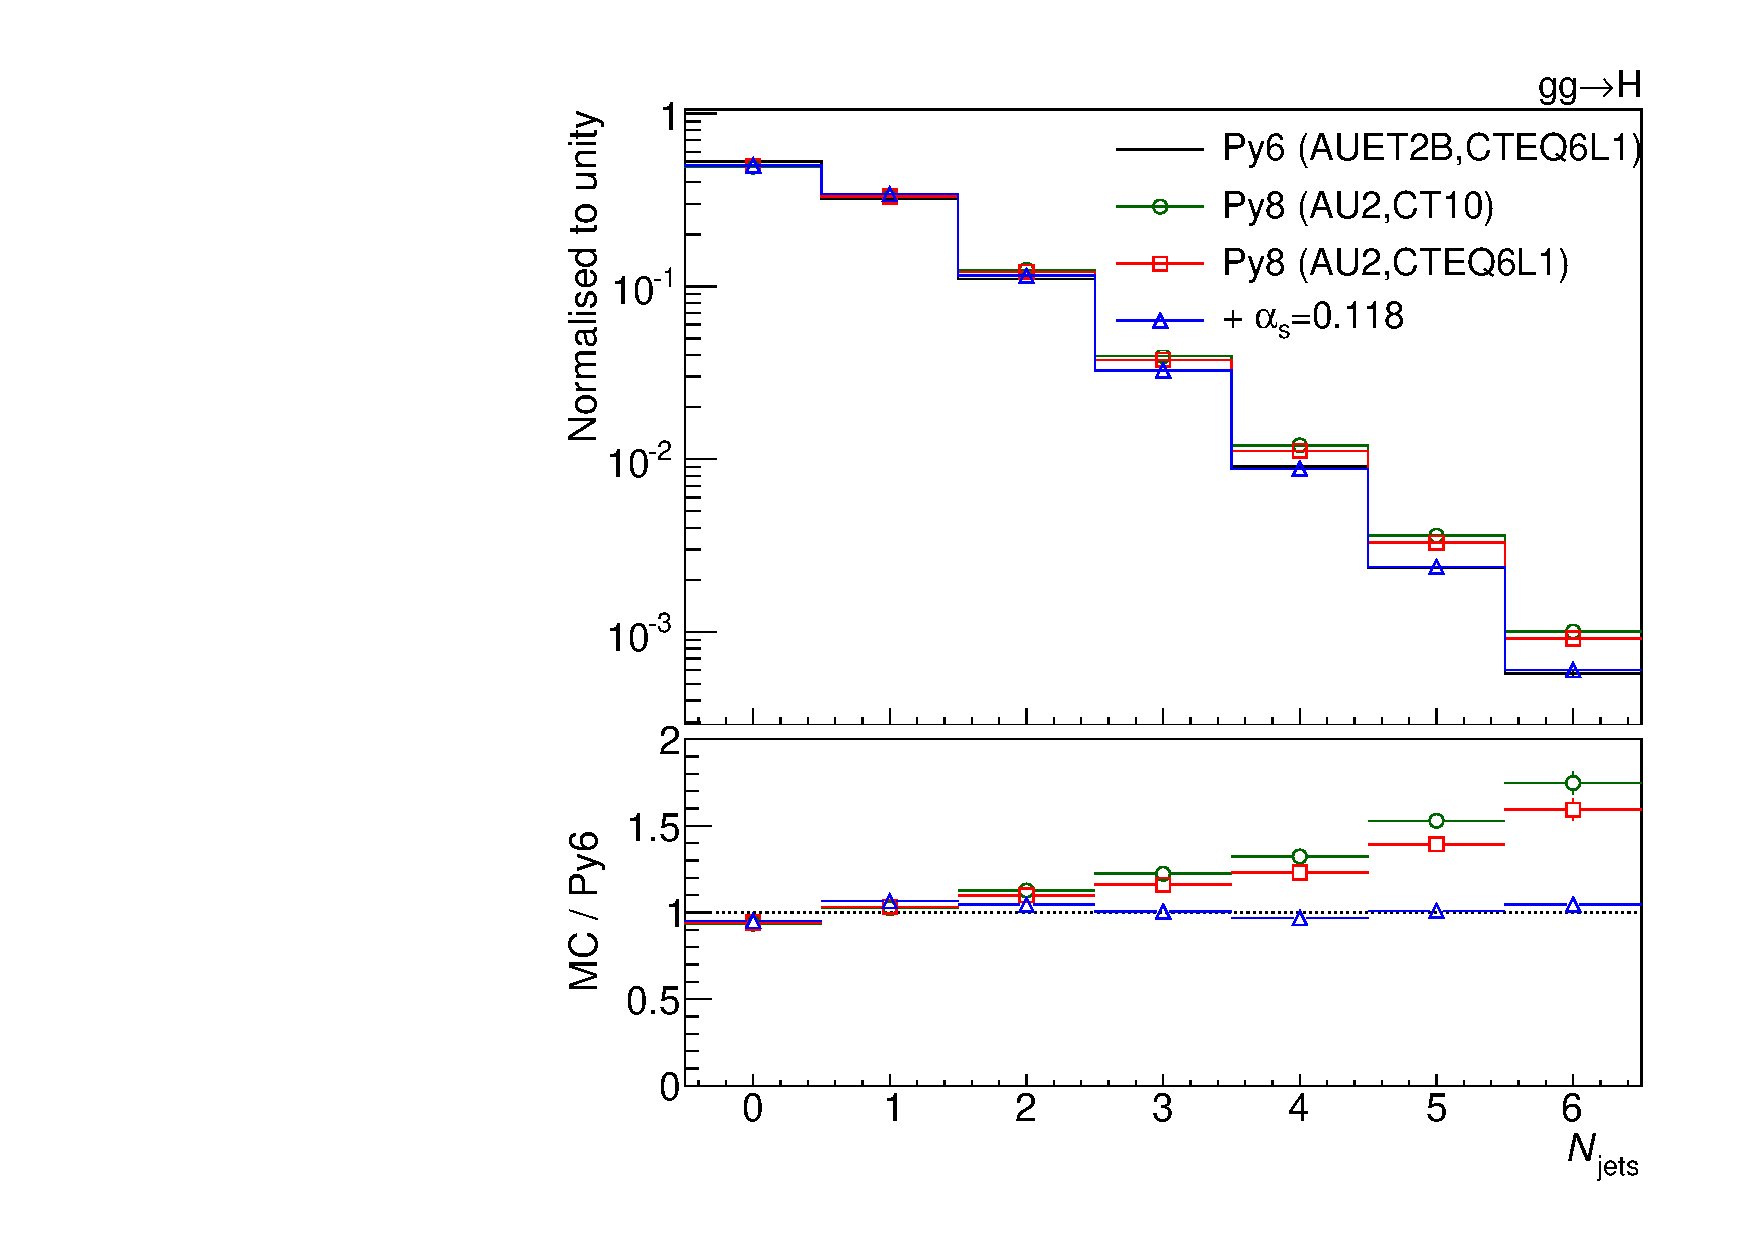
\includegraphics[width=\smallfigwidth]{tex/signal/matching}
	\caption{Jet multiplicity produced by \meps{\powhegbox}{\pythia{8}} with a selection 
	of shower tunes. The green circles is the tune used in the analysis. The red squares 
	change the parton shower PDFs from CT10 to CTEQ6L1. The blue triangles additionally 
	change the parton shower $\alphaS\parenths{\mZ}$ from 0.137 to 0.118 (in agreement 
	with \powhegbox). \meps{\powhegbox}{\pythia{6}} is shown in black for reference.}
	\label{fig:signal:matching}
\end{figure}

Identification of poor matching between \powhegbox and the \pythia{8} parton shower 
program has led to improvements in the latest round of MC tuning \cite{ATLAS:tune:2013}.
